%!TEX root = ../template.tex
%%%%%%%%%%%%%%%%%%%%%%%%%%%%%%%%%%%%%%%%%%%%%%%%%%%%%%%%%%%%%%%%%%%%
%% appendix2.tex
%% NOVA thesis document file
%%
%% Chapter with example of appendix with a short dummy text
%%%%%%%%%%%%%%%%%%%%%%%%%%%%%%%%%%%%%%%%%%%%%%%%%%%%%%%%%%%%%%%%%%%%
\chapter{Other Relevant Graphs}
\label{app:results}

    
    
        \begin{figure}[h]
        \centering
        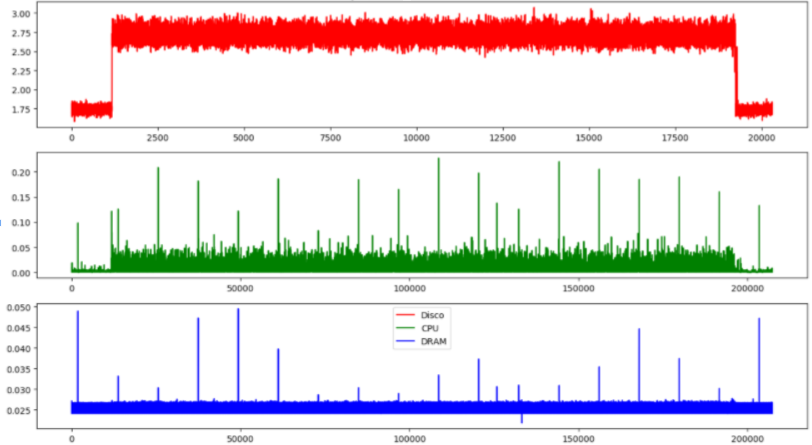
\includegraphics[width=1\columnwidth]{results/grafostempo/mysql5m.png}
        \caption{MySQL energy behavior during a 5 minutes benchmark}
        \label{fig:mysqltime5}
    \end{figure}
    
            \begin{figure}[h]
        \centering
        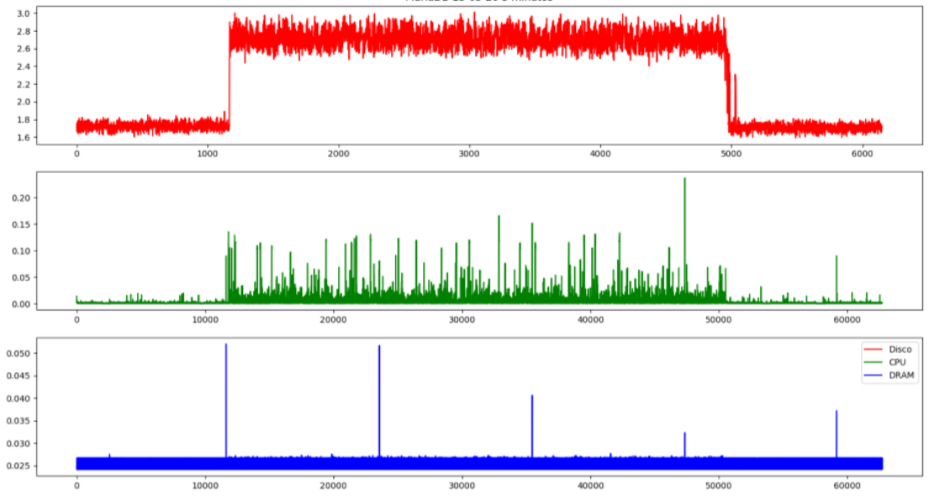
\includegraphics[width=1\columnwidth]{results/grafostempo/MariaDB.png}
        \caption{MariaDB energy behavior during a 5 minutes benchmark}
        \label{fig:mariadbtime5m}
    \end{figure}
        
    \begin{figure}[h]
        \centering
        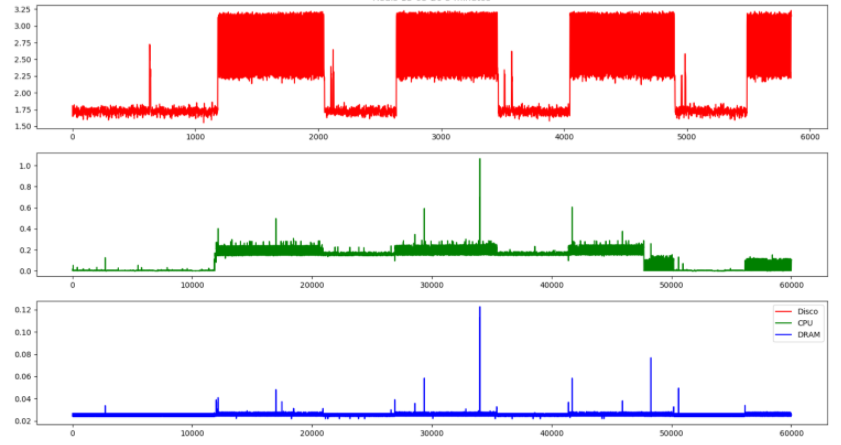
\includegraphics[width=1\columnwidth]{results/grafostempo/Redis5m.png}
        \caption{Redis energy behavior during a 5 minutes benchmark}
        \label{fig:redistime5m}
    \end{figure}
    
    
        
    \begin{figure}[h]
        \centering
        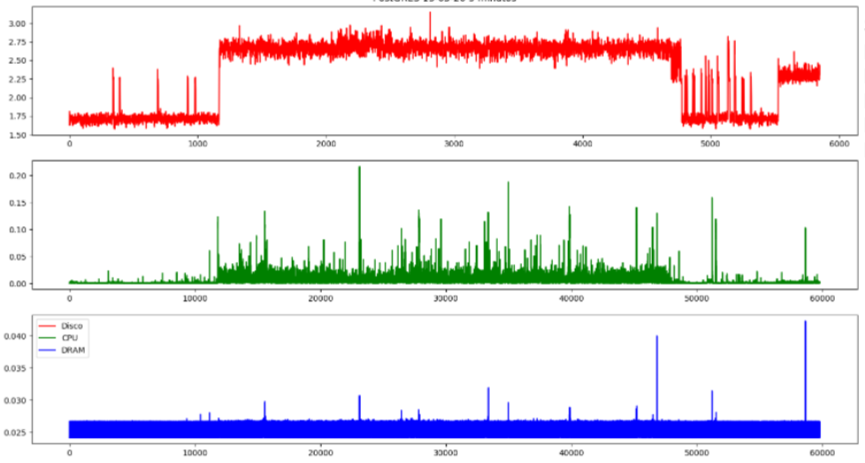
\includegraphics[width=1\columnwidth]{results/grafostempo/postgres5m.png}
        \caption{Postgres energy behavior during a 5 minutes benchmark}
        \label{fig:PostGrestime5m}
    \end{figure}
    

    \begin{figure}[h]
\centering
        \centering
        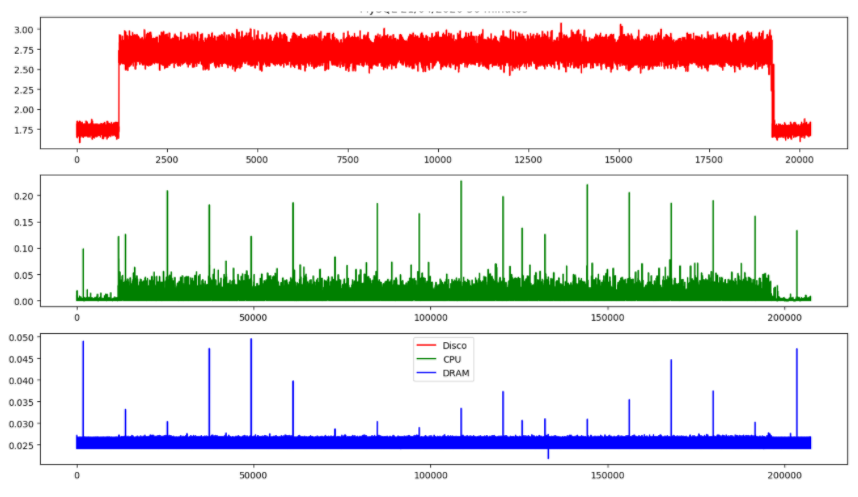
\includegraphics[width=1\columnwidth]{results/grafostempo/mysql10m.png}
        \caption{MySQL energy behavior during a 30 minutes benchmark}
        \label{fig:mysqltime}
    \end{figure}
    
        
    \begin{figure}[h]
        \centering
        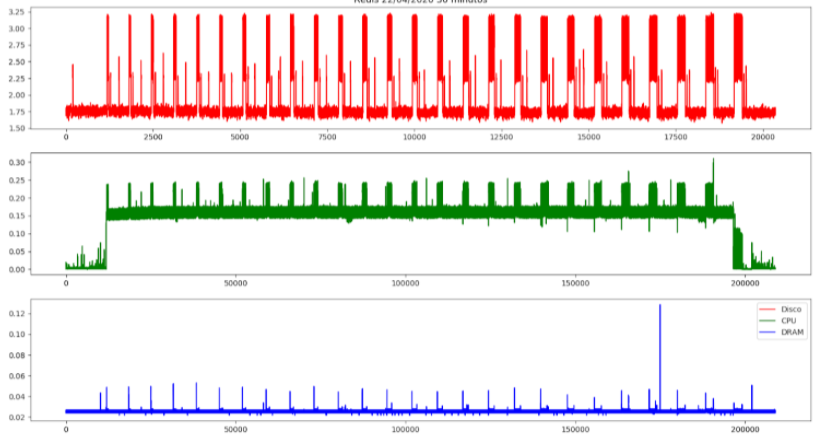
\includegraphics[width=1\columnwidth]{results/grafostempo/redis10m.png}
        \caption{Redis energy behavior during a 30 minutes benchmark}
        \label{fig:redistime30m}
    \end{figure}
    
    
        
    \begin{figure}[h]

        \centering
        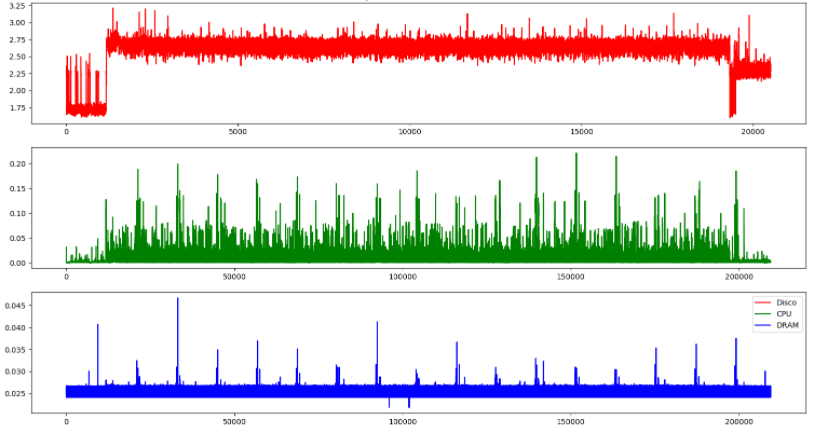
\includegraphics[width=1\columnwidth]{results/grafostempo/postgres10m.png}
        \caption{Postgres energy behavior during a 30 minutes benchmark}
        \label{fig:PostGrestime30m}
    \end{figure}
